\documentclass[a4paper,12pt]{article}
\usepackage[english]{babel}
\usepackage[utf8]{inputenc}
\usepackage[T1]{fontenc}
\usepackage{amsmath}
\usepackage{amsthm}
\usepackage{amsfonts}
\usepackage{amssymb}
\usepackage{graphicx}
\usepackage{hyperref}
\usepackage{enumitem}
\usepackage{float}
\usepackage{booktabs}
\usepackage{CJKutf8}
\usepackage[colorinlistoftodos]{todonotes}
\usepackage[left=1.50cm, right=1.50cm, top=1.20cm]{geometry}
\linespread{1.5}
\usepackage{algorithm}
\usepackage{algpseudocode}
\usepackage{tikz}
\usetikzlibrary{matrix, positioning, fit}
\usepackage{listings}
\lstset{upquote=true}


\title{LC741---750}
\author{SS}
\date{November 2018}

\begin{document}

\maketitle

\section{741 --- Cherry Pickup}
In a $N \times N$ grid representing a field of cherries, each cell is one of three possible integers.
\begin{itemize}
    \item 0 means the cell is empty, so you can pass through;
    \item 1 means the cell contains a cherry, that you can pick up and pass through;
    \item $-1$ means the cell contains a thorn that blocks your way.
\end{itemize}
Your task is to collect maximum number of cherries possible by following the rules below:
\begin{itemize}
    \item Starting at the position $(0, 0)$ and reaching $(N-1, N-1)$ by moving right or down through valid path cells (cells with value 0 or 1);
    \item After reaching $(N-1, N-1)$, returning to $(0, 0)$ by moving left or up through valid path cells;
    \item When passing through a path cell containing a cherry, you pick it up and the cell becomes an empty cell (0);
    \item If there is no valid path between $(0, 0)$ and $(N-1, N-1)$, then no cherries can be collected
\end{itemize}
\paragraph{Example 1:}
\begin{flushleft}
\textbf{Input}:
\[
G = \begin{array}{rrr}
0 & 1 &  -1 \\
1 & 0 & -1 \\
1 & 1 & 1
\end{array}
\]
\textbf{Output}: 5
\\
\textbf{Explanation}:
\\
The player started at $(0, 0)$ and went down, down, right right to reach $(2, 2)$.
\\
4 cherries were picked up during this single trip, and the matrix becomes
\[
G = \begin{array}{rrr}
0 & 1 &  -1 \\
0 & 0 & -1 \\
0 & 0 & 0
\end{array}
\]
Then, the player went left, up, up, left to return home, picking up one more cherry.
The total number of cherries picked up is 5, and this is the maximum possible.
\end{flushleft}
\subsection{Dynamic Programming}
First of all, greedy method does not work here. The reason is that maximizing the first one-way does \textbf{NOT} guarantee that we can get overall maximum number of cherries for round-trip. In the first one-way picking, we are following only the shortest path. Therefore, we may neglect some positions that would give more cherries when going back.
\par
For example, in the following grid
\begin{figure}[H]
\centering
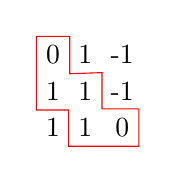
\begin{tikzpicture}
\matrix (m) [matrix of nodes]
{
0 & 1 & -1 \\
1 & 1 & -1 \\
1 & 1 & 0 \\
};
\draw [color=red](m-1-1.north west)--(m-2-1.south west)--(m-2-2.south west)--(m-3-2.south west)--(m-3-3.south east)--(m-3-3.north east)--(m-3-2.north east)--(m-2-2.north east)--(m-1-1.south east)--(m-1-1.north east)--cycle;
\end{tikzpicture}
\end{figure}
If the first round one-way shortest path goes along the red path for getting maximum 3 cherries, it splits the remaining 2 cherries into opposite sides of the diagonal which is impossible for round trip to pick up all cherries. 
\par
Therefore, we have to plan the round trip altogether. Note that the path direction is irrelevant to the problem and we are forced to move only on shortest paths.
\par
We can imagine two persons $p_1$ and $p_2$ are at $(0,0)$ during start. Then they both move by taking different path to $(N-1, N-1)$. After $t$ steps, $p_1$ is in position $(r_1,c_1)$ and $p_2$ in $(r_2, c_2)$. Both positions will have $r_1+c_1=r_2+c_2=t$. Then, $r_2 = r_1 + c_1 - c_2$, which means $r_1,c_1,c_2$ uniquely determine $p_1, p_2$ who have walked the same $t = r_1+c_1$ number of steps. This is suitable for dynamic programming quite nicely.
\par
Suppose $F[r_1][c_1][c_2]$ be the maximum number of cherries obtained by two persons $p_1$ and $p_2$ who are starting at $(r_1, c_1)$ and $(r_2, c_2)$ respectively, and are walking towards $(N-1, N-1)$ by picking up cherries, where $r_2 = r_1+c_1-c_2$.
\par
If $G[r_1][c_1] \neq -1$ and $G[r_2][c_2] \neq -1$, then $F[r_1][c_1][c_2]$ is $(G[r_1][c_1] + G[r_2][c_2])$, plus the maximum of $F[r_1+1][c_1][c_2]$, $F[r_1][c_1+1][c_2]$, $F[r_1+1][c_1][c_2+1]$ and $F[r_1][c_1+1][c_2+1]$. We should also be careful to not double count in case when $p_1$ and $p_2$ are in the same position, i.e., $(r_1, c_1) = (r_2, c_2)$.
\par
Why do we need to plus the 
\[
\max(F[r_1+1][c_1][c_2], F[r_1][c_1+1][c_2], F[r_1+1][c_1][c_2+1], F[r_1][c_1+1][c_2+1])
\]
The reason is these four values corresponds to the 4 possibilities for $p_1$ and $p_2$ moving down and right:
\begin{enumerate}
\item $p_1$ go \textbf{down} and $p_2$ go \textbf{down}: $F[r_1+1][c_1][c_2]$ since $r_2 \gets r_1 + 1 +c_1 -c_2 = (r_1+c_1-c_2) + 1 = r_2+1$
\item $p_1$ go \textbf{right} and $p_2$ go \textbf{down}: $F[r_1][c_1+1][c_2]$ since $r_2 \gets r_1 + c_1 + 1 -c_2 = (r_1+c_1-c_2) + 1 = r_2+1$
\item $p_1$ go \textbf{down} and $p_2$ go \textbf{right}: $F[r_1+1][c_1][c_2+1]$ since $r_2$ is unchanged because $r_2= r_1 + c_1 + 1 -c_2 - 1 = (r_1+c_1-c_2) = r_2$
\item $p_1$ go \textbf{right} and $p_2$ go \textbf{right}: $F[r_1][c_1+1][c_2+1]$ since $r_2$ is unchanged because $r_2= r_1 + c_1 + 1 -c_2 - 1 = (r_1+c_1-c_2) = r_2$
\end{enumerate}
\subsubsection{Code}
Inputs of this procedure are
\begin{itemize}
\item $G, N$ --- The input $N\times N $ grid
\end{itemize}
\setcounter{algorithm}{0}
\begin{algorithm}[H]
\caption{Recursive Dynamic Programming Approach}
\begin{algorithmic}[1]
\Procedure{CherryPickup}{$G, N$}
\State $F$ as $F[0][0][0] = \ldots = F[N-1][N-1][N-1]:= -1$ \Comment The memo \texttt{dp} array.
\State $\nu: = \Gamma(F, G, N, 0, 0, 0)$ \Comment Starting from $p_1, p_2$ both are at $(0,0)$ [\ref{741gf}]
\State \Return $\max(0, \nu)$ \Comment When no path from $(0,0)$ to $(N-1, N-1)$, $\nu < 0$
\EndProcedure
\end{algorithmic}
\end{algorithm}

Input parameters of the following recursive function $\Gamma$ include:
\begin{itemize}
\item $F$ --- The memo array
\item $G, N$ --- The input grid $N\times N$ grid
\item $r_1, c_1, c_2$ --- The position $(r_1, c_1)$ and $(r_2, c_2)$ of the two persons, where $r_2 = r_1+c_1-c_2$
\end{itemize}
\begin{algorithm}[H]
\caption{Recursive Function With Memo Array}
\label{741gf}
\begin{algorithmic}[1]
\Function{$\Gamma$}{$F, G, N, r_1, c_1, c_2$}
\State $r_2 := r_1+c_1-c_2$ \Comment $r_2$ is uniquely determined by $r_1,c_1,c_2$
\If{$r_1 = N$ \textbf{and} $c_1 = N$ \textbf{and} $r_2 = N$ \textbf{and} $c_2 = N$} \Comment Boundary case
\State \Return -1;
\EndIf
\If{$G[r_1][c_1] = -1$ \textbf{and} $G[r_2][c_2] = -1$} \Comment Cannot get to these positions
\State \Return -1;
\EndIf
\If{$r_1=N-1$ \textbf{and} $c_1 = N-1$} \Comment $p_1$ arrive at $(N-1, N-1)$ and get the cherry here.
\State \Return $G[r_1][c_1]$
\EndIf
\If{$F[r_1][c_1][c_2] \neq -1$} \Comment Memo $F$ has value which is different from initial value \label{741gfnote0}
\State \Return $F[r_1][c_1][c_2]$ \Comment  Return this value directly
\EndIf
\State $\mu:=G[r_1][c_1]$ \Comment Get cherry at $(r_1, c_1)$
\If{$c_1\neq c_2$} \Comment $p_1$ and $p_2$ are not at same positions.
\State $\mu\gets \mu+G[r_2][c_2]$ \Comment Get cherry at $(r_2, c_2)$
\EndIf
\State $f_1 := \Gamma(F, G, N, r_1+1, c_1, c_2)$ \Comment $p_1$ go down  and $p_2$ go down
\State $f_2 := \Gamma(F, G, N, r_1+1, c_1, c_2+1)$ \Comment $p_1$ go down  and $p_2$ go right
\State $f_3 := \Gamma(F, G, N, r_1, c_1+1, c_2)$ \Comment $p_1$ go right  and $p_2$ go down
\State $f_4 := \Gamma(F, G, N, r_1, c_1+1, c_2+1)$ \Comment $p_1$ go right  and $p_2$ go right
\State $\gamma := \max(f_1,f_2,f_3,f_4)$ \Comment Get the maximum of these 4 moves
\If{$\gamma=-1$} \Comment No way to $(N-1), (N-1)$ from $(r_1, c_1)$ and $(r_2, c_2)$
\State $F[r_1][c_1][c_2] = -100$ \Comment Set $F[r_1][c_1][c_2]$ to a different value $-100$ \label{741gfnote1}
\State \Return $-100$
\EndIf
\State $\mu\gets \mu + \gamma$
\State $F[r_1][c_1][c_2] =\mu$ \Comment Save to memo array
\State \Return $\mu$
\EndFunction
\end{algorithmic}
\end{algorithm}
The reason we set $F[r_1][c_1][c_2]$ to $-100$ at line [\ref{741gfnote1}] is that we need to return immediately if we find that the two persons cannot arrive $(N-1, N-1)$. However, $F[r_1][c_1][c_2]$ has initial value $-1$. So we use a different value $-100$ to differentiate from the initial value. Otherwise, if we still return $-1$ in this case, line [\ref{741gfnote0}] will ignore and continue to test. The result is a infinite loop.
\subsection{Iterative Dynamic Programming}
Like in recursive dynamic programming approach, Suppose $r_1+c_1=r_2+c_2=t$, we can iterate $t$ from 1 to $2\times N-2$. Why is maximum of $t$ $2\times N-2$? To arrive $(N-1,N-1)$ from $(0,0)$ by taking right and down only, we will take $N-1$ steps along column direction and $N-1$ steps along row direction. At step $t$, we define a \texttt{dp} array $F[c_1][c_2]$ as the most cherries that we can pick up for two persons going from $(0, 0)$ to $(r_1, c_1)$ and $(0, 0)$ to $(r_2, c_2)$, where $r_1 = t-c_1, r_2 = t-c_2$. Then we update $\Delta[c_1][c_2]$ as the sum of 3 values, which are 
\begin{enumerate}
\item The number of cherry at $(r_1, c_1)$
\item The number of cherry at $(r_2, c_2)$ if $c_1\neq c_2$, i.e., the two persons are not at same position.
\item The maximum of $\Delta[c_1][c_2]$, $\Delta[c_1][c_2-1]$, $\Delta[c_1-1][c_2]$ and $\Delta[c_1-1][c_2-1]$. $\Delta[c_1][c_2]$ is similar \texttt{dp} array in the last step $t-1$. Which implicitly get maximum of values in $(r_1-1, c_1)$, $(r_1, c_1-1)$, $(r_2-1, c_2)$ and $(r_2, c_2-1)$
\end{enumerate}
In each iteration of step $t$, we need to determine the starting and ending column indexes. Because $0\leq c\leq N-1$,
\begin{itemize}
\item If $t\leq N-1$, we will have $0\leq c \leq t$ hence $0\leq r=t-c\leq t$
\item If $t> N-1$, then $c \leq t-(N-1)$. Otherwise $r=t-c >N-1$, it is impossible. Therefore $t-(N-1) \leq c \leq N-1$, then $t-(N-1) \leq r=t-c\leq N-1$
\end{itemize}
In summary, the starting and ending columns indexes will be $\max(0, t-(N-1))$ and $\min(N-1, t)$.
\subsubsection{Code}
\begin{algorithm}[H]
\caption{Iterative Dynamic Programming Approach}
\begin{algorithmic}[1]
\Procedure{CherryPickup}{$G, N$}
\State $\Delta$ as $\Delta[0][0] =\ldots = \Delta[N-1][N-1]:=-1$ \Comment The \texttt{dp} array
\State $\Delta[0][0]\gets G[0][0]$
\For{$t:=1$ \textbf{to} $2\times N-2$} \label{741itdpfor1}
\State $F$ as $F[0][0] = \ldots = F[N-1][N-1] := -1$ \Comment The \texttt{dp} array in current step $t$
\State $\alpha:=\max(0, t-(N-1))$ \Comment The starting column index
\State $\beta:=\min(N-1, t)$ \Comment The ending column index
\For{$c_1:=\alpha$ \textbf{to} $\beta$} \label{741iterfor1}
\For{$c_2:=\alpha$ \textbf{to} $\beta$} \label{741iterfor2}
\State $r_1:=t-c_1$
\State $r_2:=t-c_2$
\If{$G[r_1][c_1] = -1$ \textbf{or} $G[r_2][c_2] = -1$} \Comment Cannot arrive at $(r_1, c_1)$ or $(r_2,c_2)$ \State \texttt{continue}
\EndIf
\State $\nu:=G[r_1][c_1]$ \Comment The cherries collected by $p_1$ in current step $t$
\If{$c_1\neq c_2$} \Comment The two persons are not at the same position
\State $\nu \gets \nu + G[r_2][c_2]$ \Comment Add the cherries collected by $p_2$ in current step $t$
\EndIf
\State $\ell:=\Delta[c_1][c_2]$ \label{741itexplain_start}
\If{$c_1 \geq 1$}
\State $\ell\gets \max(\ell, \Delta[c_1-1][c_2]$
\EndIf
\If{$c_2 \geq 1$}
\State $\ell\gets \max(\ell, \Delta[c_1][c_2-1]$
\EndIf
\If{$c_1 \geq 1$ \textbf{and} $c_2 \geq 1$}
\State $\ell\gets \max(\ell, \Delta[c_1-1][c_2-1]$
\EndIf \label{741itexplain_end}
\algstore{741iter}
\end{algorithmic}
\end{algorithm}
\begin{algorithm} [H]
\begin{algorithmic}[1]
\algrestore{741iter}
\If{$\ell = -1$} \Comment $p_1, p_2$ cannot get cherries at last step $t-1$
\State \texttt{continue}
\EndIf
\State $F[r_1][c_1] \gets \max(F[r_1][c_1], \nu + \ell)$ \Comment Update cherries got at step $t$ by $p_1$ and $p_2$
\EndFor \Comment End[\ref{741iterfor1}]
\EndFor \Comment End[\ref{741iterfor2}]
\State $F\leftrightarrow \Delta$ \Comment Swap $F$ and $\Delta$ to update $\Delta$ to step $t$
\EndFor \Comment End[\ref{741itdpfor1}]
\State \Return $\max(0, \Delta[N-1][N-1])$ \Comment $\Delta[N-1][N-1]<0$ means cannot reach $(N-1, N-1)$
\EndProcedure
\end{algorithmic}
\end{algorithm}
From Line [\ref{741itexplain_start}] to [\ref{741itexplain_end}], we actually get maximum cherries collected at $(r_1-1,c_1)$, $(r_1,c1-1)$ by $p_1$ and $(r_2-1,c_2)$, $(r_2,c1-2)$ by $p_2$ in the last step $t-1$.
\begin{itemize}
    \item $\Delta$ records the cherries collected at each position in the last step $t-1$.
    \item The cherries collected at $(r_1-1, c_1)$ by $p_1$ and $(r_2-1, c_2)$ by $p_2$ in the last step $t- 1$ is $\Delta[c_1][c_2]$ since $t-1-c_1 = r_1-1$ and $t-1-c_2 = r_2-1$
    \item The cherries collected at $(r_1, c_1-1)$ by $p_1$ and $(r_2-1, c_2)$ by $p_2$ in the last step $t- 1$ is $\Delta[c_1-1][c_2]$ since $t-1-(c_1-1) = r_1$ and $t-1-c_2 = r_2-1$
    \item The cherries collected at $(r_1, c_1)$ by $p_1$ and $(r_2, c_2-1)$ by $p_2$ in the last step $t- 1$ is $\Delta[c_1][c_2-1]$ since $t-1-c_1 = r_1-1$ and $t-1-(c_2-1) = r_2$
    \item The cherries collected at $(r_1, c_1-1)$ by $p_1$ and $(r_2, c_2-1)$ by $p_2$ in the last step $t- 1$ is $\Delta[c_1-1][c_2-1]$ since $t-1-(c_1-1) = r_1$ and $t-1-(c_2-1) = r_2$
\end{itemize}

\section{743 --- Network Delay Time}
There are $N$ network nodes, labelled 1 to $N$.
\par
Given times, a list of travel times as directed edges $T[i] = (u, v, w)$, where $u$ is the source node, $v$ is the target node, and $w$ is the time it takes for a signal to travel from source to target.
\par
Now, we send a signal from a certain node $K$. How long will it take for all nodes to receive the signal? If it is impossible, return $-1$.
\paragraph{Note:}
\begin{flushleft}
$N$ will be in the range $[1, 100]$.
\\
$K$ will be in the range $[1, N]$.
\\
The length of times will be in the range $[1, 6000]$.
\\
All edges $T[i] = (u, v, w)$ will have $1 \leq u, v \leq N$ and $1 \leq w \leq 100$.
\end{flushleft}
\subsection{Dijkstra Algorithm}
This is actually a dijkstra shortest path algorithm. For Dijkstra's algorithm, it is always recommended to use heap (or priority queue) as the required operations (extract minimum and decrease key) match with speciality of heap (or priority queue). However, the problem is, priority queue in C++ does not support decrease key. To resolve this problem, do not update a key, but insert one more copy of it. So we allow multiple instances of same vertex in priority queue. This approach does not require decrease key operation and has below important properties.
\par
Whenever distance of a vertex is reduced, we add one more instance of vertex in the priority queue. Even if there are multiple instances, we only consider the instance with minimum distance and ignore other instances.
\par
The time complexity remains $O(E\lg V))$ as there will be at most $O(E)$ vertices in priority queue and $O(\lg E)$ is same as $O(\lg V)$
\par
Below is algorithm based on above idea.
\begin{enumerate}
    \item Initialize distances of all vertices as infinite.
    \item Create an empty priority queue $Q$.  Every item of $Q$ is a pair (vertex, weight). 
    \item Insert source vertex into $Q$ and make its distance as 0.
    \item While $Q$ is empty
    \begin{enumerate}
        \item Extract minimum distance vertex from $Q$. Let the extracted vertex be $u$.
        \item Loop through all adjacent of $u$. If we find $D[v] > D[u] + W(u, v)$, then we update the distance of v $D[v]$ as $D[u] + W(u,v)$, i.e. the distance of $u$ plus the distance from $u$ to $v$. After that, we insert $(v, D[v])$ into $Q$.
    \end{enumerate}
\end{enumerate}
\subsection{Code}
Inputs of the following algorithm include
\begin{itemize}
\item $T$ --- The input times array
\item $L$ --- The length of $T$
\item $N$ --- The number of nodes
\item $K$ --- The starting node
\end{itemize}
\begin{algorithm}[H]
\caption{Dijkstra Algorithm With Priority Queue}
\begin{algorithmic}[1]
\Procedure{NetworkDelayTime}{$T, L, N, K$}
\State $D$ as $D[0]=\ldots=D[N]:=\infty$
\State $D[K]\gets 0$ \Comment The source node distance is zero
\State $M:=\emptyset$ \Comment A hash map for each node $v$ and its adjacent nodes
\For{$i:=0$ \textbf{to} $L-1$}
\State $u:= T[i][0]$
\State $([u, [\ldots]]\;|M) \gets ([u, [\ldots, i]]\;|M)$ \Comment Insert source node and the index in $T$ into $M$
\EndFor
\State $Q:=\emptyset$ \Comment Initialize priority queue $Q$ as empty
\State $Q\gets Q + (K, 0)$ \Comment Push $K$ into the queue
\While{$Q\neq \emptyset$}
\State $(u, d):= Q[0]$ \Comment Get the top of $Q$
\State $Q\gets Q \setminus Q[0]$ \Comment Pop top of $Q$
\For{$k \in M[u]$} \Comment Iterate each adjacent vertex of $u$
\State $v:= T[k][1]$ \Comment The destination node is the 2nd element of $T[k]$
\State $d:=T[k][2]$ \Comment The distance is the 3rd element of $T[k]$
\If{$D[v] > D[u] + d$}
\State $D[v]\gets D[u] + d$ \Comment Update $D[v]$
\State $Q\gets Q + D[v]$ \Comment Push into $Q$
\EndIf
\EndFor
\EndWhile
\algstore{743algo}
\end{algorithmic}
\end{algorithm}

\begin{algorithm}[H]
\begin{algorithmic}[1]
\algrestore{743algo}
\State $\Bar{D}:= -\infty$ \Comment The returned shorted path distance
\For{$i:=1$ \textbf{to} $N$}
\If{$D[i] = \infty$} \Comment Node $i$ cannot be reached
\State \Return $-1$
\EndIf
\State $\Bar{D} \gets \max(\Bar{D}, D[i]) $ \Comment The maximum of $D[i]$
\EndFor
\State \Return $\Bar{D}$
\EndProcedure
\end{algorithmic}
\end{algorithm}

\section{742 --- Closest Leaf in a Binary Tree}
Given a binary tree where every node has a unique value, and a target key $k$, find the value of the nearest leaf node to target $k$ in the tree.
\par
Here, nearest to a leaf means the least number of edges travelled on the binary tree to reach any leaf of the tree. Also, a node is called a leaf if it has no children.
\par
In the following examples, the input tree is represented in flattened form row by row. The actual root tree given will be a \texttt{TreeNode} object.
\paragraph*{Example}
\begin{flushleft}
\textbf{Input}: $r=[1,3,2], k=1$
\begin{figure}[H]
\begin{tikzpicture}
[bsarrow/.style={->,>=stealth}]
\node(){};
\node(1) {$1$};
\node(2) [below = 3mm of 1, xshift = -5mm]{$2$};
\node(3) [below = 3mm of 1, xshift = 5mm]{$3$};
\draw[bsarrow] (1) -- (2);
\draw[bsarrow] (1) -- (3);
\end{tikzpicture}
\end{figure}
\textbf{Output}: 2 (or 3)
\\
\textbf{Explanation}: Either 2 or 3 is the nearest leaf node to the target of 1.
\end{flushleft}
\paragraph*{Example}
\begin{flushleft}
\textbf{Input}: $R = [1], k=1$
\\
\textbf{Output}: 1
\\
\textbf{Explanation}: The nearest leaf node is the root node itself.
\end{flushleft}
\paragraph*{Example}
\begin{flushleft}
\textbf{Input}: $R = [1,2,3,4,\varnothing,\varnothing,\varnothing,5,\varnothing,6], k = 2$
\begin{figure}[H]
\begin{tikzpicture}
[bsarrow/.style={->,>=stealth}]
\node(){};
\node(1) {$1$};
\node(2) [below = 3mm of 1, xshift = -5mm]{$2$};
\node(3) [below = 3mm of 1, xshift = 5mm]{$3$};
\node(4) [below = 3mm of 2, xshift = -5mm]{$4$};
\node(5) [below = 3mm of 4, xshift = -5mm]{$5$};
\node(6) [below = 3mm of 5, xshift = -5mm]{$6$};
\draw[bsarrow] (1) -- (2);
\draw[bsarrow] (1) -- (3);
\draw[bsarrow] (2) -- (4);
\draw[bsarrow] (4) -- (5);
\draw[bsarrow] (5) -- (6);
\end{tikzpicture}
\end{figure}
\textbf{Output}: 3
\\
\textbf{Explanation}: The leaf node with value 3 (and not the leaf node with value 6) is nearest to the node with value 2.
\end{flushleft}

\section{745 --- Prefix and Suffix Search}
Given many words $W$, $W[i]$ has weight $i$.
\par
Design a class \texttt{WordFilter} that supports one function:
\begin{lstlisting}[backgroundcolor=\color{blue!80!green!10}, keywordstyle=\bfseries\color{green!40!black}, commentstyle=\itshape\color{purple!40!black},language=Java]
WordFilter.f(String prefix, String suffix)
\end{lstlisting}
It will return the word with given \texttt{prefix} (denoted as $\alpha$) and \texttt{suffix} (denoted as $\beta$) with maximum weight. If no word exists, return $-1$.
\paragraph{Examples:}
\begin{flushleft}
\begin{lstlisting}[backgroundcolor=\color{blue!80!green!10}, keywordstyle=\bfseries\color{green!40!black}, commentstyle=\itshape\color{purple!40!black},language=Java]
WordFilter(["apple"])
WordFilter.f("a", "e") // returns 0
WordFilter.f("b", "") // returns -1
\end{lstlisting}
\end{flushleft}
\paragraph{Note:}
\begin{flushleft}
$|W|$ is in range $[1, 15000]$.
\\
For each test case, up to $|W|$ queries may be made.
\\
$|W[i]|$ is in range $[1, 10]$.
\\
\texttt{prefix} $\alpha$, \texttt{suffix} $\beta$ have lengths in range $[0, 10]$.
\\
$|W[i]$ and $\alpha$, $\beta$ queries consist of lowercase letters only.
\end{flushleft}
\subsection{Pair Trie}
Say we are inserting the word \texttt{apple}. We could insert $(a, e)$, $(p, l)$, $(p, p)$, $(l, p)$ and $(e, a)$ into the trie. Then, if we had equal length queries like $\alpha = \texttt{ap}$, $\beta = \texttt{le}$, we could find the node $t(a, e)(p, l)$ in the trie. This seems promising.
\par
What about queries that are not equal? We should just insert them like normal. For example, to capture a case like $\alpha = \texttt{app}$, $\beta = \texttt{e}$, we could create nodes $t(a, e)(p, \varnothing)(p, \varnothing)$.
\par
After inserting these pairs into the trie, the searches are straightforward.
\par
Take \texttt{apple} as the example, we will insert the following strings into the trie
\begin{itemize}
\item \texttt{apple}, \texttt{pple}, \texttt{ple}, \texttt{le} and \texttt{e}
\item \texttt{elppa}, \texttt{lppa}, \texttt{ppa}, \texttt{pa} and \texttt{a}
\item \texttt{ae}, \texttt{pl}, \texttt{pp}, \texttt{lp} and \texttt{ea}
\end{itemize}
Notice, since \texttt{apple} covers all prefix, therefore, we do not need to put \texttt{ap},\texttt{app}, \texttt{appl} into the trie.
\subsubsection{Code}
In real implementation, we can transform two characters into a integer. For example, for the word \texttt{apple}, when we want to insert node $(a,e)$, first we transform into a integer $i$ by this formula $v=(\texttt{ascii}(a) - \texttt{ascii}(a) + 1) \times 27 + (\texttt{ascii}(e)-\texttt{ascii}(a) + 1$ since the problem only allows lower case letters.
\par
When doing the search for given prefix and suffix, we start from the begin of prefix and end of suffix. If the pointers to prefix and suffix are valid, we get the integer of both characters from prefix and suffix by formula above and search in the tire. Otherwise, we get integer from the character only from the pointer that still is valid to search in the trie. If both pointers are invalid, we end the search.
\par
The constructor procedure take the words array $W$ which has a length $N$, and create a trie tree with root $T$. The trie node structure is defined as following
\begin{lstlisting}[backgroundcolor=\color{blue!80!green!10}, keywordstyle=\bfseries\color{green!40!black}, commentstyle=\itshape\color{purple!40!black},language=C++]
struct TrieNode
{
	unordered_map<int, TrieNode*> Z;
	int W;
	TrieNode ():weight(0){}
};
\end{lstlisting}
\setcounter{algorithm}{0}
\begin{algorithm}[H]
\caption{Pair Trie Approach: Contructor}
\begin{algorithmic}[1]
\Procedure{WordFilter}{$W, N$}
\State Create a new trie node $T$ as the root
\For{$i:=0$ \textbf{to} $N-1$} \label{745CtorFor1}
\State $w:=W[i]$ \Comment The current word $w$
\For{$w_i:=0$ \textbf{to} $|w|-1$} \label{745CtorFor2}
\State $t:=T$ \Comment Starting with the root 
\For{$\delta:=w_i$ \textbf{to} $|w|-1$} \Comment From left to right \label{745CtorFor3}
\State $ v:= (w[\delta] - \texttt{ascii}(a) + 1)\times 27$ \Comment Convert to integer from char type \label{745algonote1}
\State $t\gets \Omega(v, t)$ \Comment Insert $v$ into $t$
\State $t_W \gets i$ \Comment Set trie node $t$'s weight $W$
\EndFor \Comment End[\ref{745CtorFor3}]
\State $t\gets T$ \Comment Reset $t$ to the root
\For{$\delta:=|w| - 1 - w_i$ \textbf{to} $0$} \Comment From right to left \label{745CtorFor4}
\State $ v:= w[\delta] - \texttt{ascii}(a) + 1$ \Comment Convert to integer from char type
\State $t\gets \Omega(v, t)$ \Comment Insert $v$ into $t$
\State $t_W \gets i$ \Comment Set trie node $t$'s weight $W$
\EndFor \Comment End[\ref{745CtorFor4}]
\State $v_1:= w[w_i] - \texttt{ascii}(a) + 1$ \Comment Covert $w[w_i]$ into integer
\State $v_2:= w[|w| - 1 - w_i] - \texttt{ascii}(a) + 1$ \Comment Convert $w[|w| - 1 - w_i]$ into integer
\State $v:=v_1\times 27+v_2$ \Comment Combine $v_1$ and $v_2$ into one integer \label{745algonote2}
\State $t\gets \Omega(v,t)$ \Comment Insert $v$  into $t$
\State $t_W \gets i$ \Comment Set trie node $t$'s weight $W$
\EndFor \Comment End[\ref{745CtorFor2}]
\EndFor \Comment End[\ref{745CtorFor1}]
\EndProcedure
\end{algorithmic}
\end{algorithm}

Function $\Omega$ insert value $v$ into the trie node $t$
\begin{algorithm}[H]
\caption{Helper Function To Insert To Trie}
\label{745insert}
\begin{algorithmic}[1]
\Function{$\Omega$}{$v, t$}
\If{$v$ is not found in $t$'s member $Z$} 
\State Insert $v$ and a new trie node $\hat{t}$ into $Z$: $Z[v]=\hat{t}$
\EndIf
\algstore{745algofunc}
\end{algorithmic}
\end{algorithm}
\begin{algorithm}[H]
\begin{algorithmic}[1]
\algrestore{745algofunc}
\State \Return $Z[v]$ \Comment Return the trie node associated with $v$
\EndFunction
\end{algorithmic}
\end{algorithm}

Function $f$ returns the maximum weight for the given prefix $\alpha$ and suffix $\beta$
\begin{algorithm}[H]
\caption{Search The Maximum Weight For Given Prefix And Suffix}
\begin{algorithmic}[1]
\Procedure{$f$}{$\alpha, \beta$}
\State $t:=T$ \Comment Starting from the trie root $T$
\State $i:=0$ \Comment The pointer to the prefix $\alpha$
\State $j:=|\beta| - 1$ \Comment The pointer to the suffix $\beta$ and is at the end of $\beta$ initially
\While{$i<|\alpha|$ \textbf{or} $j \geq 0$} \label{745fwhile1}
\State $v_1:=0, v_2:=0$
\If{$i < |\alpha|$}
\State $v_1:\gets\alpha[i] - \texttt{ascii}(a) + 1$ \Comment Convert $\alpha[i]$ to integer $v_1$
\EndIf
\If{$j \geq 0$}
\State $v_2\gets\beta[j] - \texttt{ascii}(a) + 1$ \Comment Convert $\beta[j]$ to integer $v_1$
\EndIf
\State $v:=v_1\times 27 + v_2$ \Comment Get the integer value of combination of $\alpha[i]$ and $\beta[j]$
\If{$v$ cannot be found in $t$}
\State \Return $-1$ \Comment $\alpha$ and/or $\beta$ is not found in given words
\Else
\State $t\gets t_{Z}[v]$ \Comment Get the trie node associated with $v$
\EndIf
\State $i\gets i+1, j\gets j-1$ \Comment Move the pointers 
\EndWhile \Comment End[\ref{745fwhile1}]
\State \Return $t_{W}$ \Comment Return the weight in current trie node $t$
\EndProcedure
\end{algorithmic}
\end{algorithm}
\subsection{Trie of Suffix Wrapped Words}
For each suffix of the word, we could insert that suffix, followed by a special character like \texttt{\#}, followed by the word, all into the trie.
\par
Take the word \texttt{apple} as the example, we will insert \texttt{\#apple}, \texttt{e\#apple}, \texttt{le\#apple}, \texttt{ple\#apple}, \texttt{pple\#apple} and \texttt{apple\#apple} into the trie. Then for a query like prefix is \texttt{ap}, suffix is \texttt{le}, we can find it by querying our trie for \texttt{le\#ap}.
\subsection{Code}
The implementation is similar to previous one. We still use the same insert function $\Omega$ [\ref{745insert}].
\begin{algorithm}[H]
\caption{Trie Of Prefix And Suffix}
\begin{algorithmic}[1]
\Procedure{WordFilter}{$W, N$}
\State Create a new trie node $T$ as the root
\State $\Omega(\texttt{ascii}(\texttt{\#}), T)$ \Comment Insert \texttt{\#} into trie
\For{$i:=0$ \textbf{to} $N-1$} \label{745Ctor1For1}
\State $w:=W[i]$ \Comment The current word $w$
\State $t:=T_Z[\texttt{ascii}(\texttt{\#})]$ \Comment Get the trie node associated with \texttt{\#} for prefix strings
\For{$i:=0$ \textbf{to} $|w|-1$} \label{745Ctor1For2}
\State $t\gets \Omega(\texttt{ascii}(w[i]), t)$ \Comment Insert $w[i]$ into $t$
\State $t_W \gets i$ \Comment Set trie node $t$'s weight $W$
\EndFor \Comment End[\ref{745Ctor1For2}]
\For{$i:=|w| - 1$ \textbf{to} $0$} \Comment From right to left \label{745Ctor1For3}
\State $t\gets T$ \Comment Reset $t$ to the root of trie
\For{$j:=i$ \textbf{to} $|w|-1$} \Comment Build suffix trie \label{745Ctor1For4}
\State $t\gets \Omega(\texttt{ascii}(w[j]), t)$ \Comment Insert $w[j]$ into $t$
\State $t_W \gets i$ \Comment Set trie node $t$'s weight $W$
\EndFor \Comment End [\ref{745Ctor1For4}]
\State $t:=\Omega(\texttt{ascii}(\texttt{\#}), T)$ \Comment Append \texttt{\#} into trie
\For{$k:=0$ \textbf{to} $|w|-1$} \Comment Append $w$ into trie \label{745Ctor1For5}
\State $t:=\Omega(\texttt{ascii}(w[k]), T)$ 
\State $t_W \gets i$ \Comment Set trie node $t$'s weight $W$
\EndFor \Comment End[\ref{745Ctor1For5}]
\EndFor \Comment End[\ref{745Ctor1For3}]
\EndFor \Comment End[\ref{745Ctor1For1}]
\EndProcedure
\end{algorithmic}
\end{algorithm}
Search function $f$ is straightforward. It will search words by the prefix $\alpha$ and suffix $\beta$ through the combined string $\alpha + \texttt{\#} + \beta$. Skip the code here. 

\section{744 --- Find Smallest Letter Greater Than Target}
Given a list of sorted characters letters $A$ containing only lowercase letters, and given a target letter target $T$, find the smallest element in the list that is larger than the given target.
\par
Letters also wrap around. For example, if the target $T$ is $z$ and letters $A = [a, b]$, the answer is $a$.
\paragraph{Examples:}
\begin{flushleft}
\textbf{Input:} $A=(c,f,j), T=a$
\\
\textbf{Output:} $c$
\\
\textbf{Input:} $A=(c,f,j), T=k$
\\
\textbf{Output:} $c$
\end{flushleft}
\paragraph{Note:}
\begin{flushleft}
letters has a length in range $[2, 10000]$.
\\
letters consists of lowercase letters, and contains at least 2 unique letters.
\\
target is a lowercase letter.
\end{flushleft}
\subsection{Binary Search}
This is the rightmost binary search. If the found index pass the end of $A$, we wrap it into the first letter of $A$


\section{746 --- Min Cost Climbing Stairs}
On a staircase, the $i$--th step has some non-negative cost $\nu[i]$ assigned (0 indexed).
\par
Once you pay the cost, you can either climb one or two steps. You need to find minimum cost to reach the top of the floor, and you can either start from the step with index 0, or the step with index 1.
\paragraph{Example 1:}
\begin{flushleft}
\textbf{Input}: $\nu = [10, 15, 20]$
\\
\textbf{Output}: 15
\\
\textbf{Explanation}: Cheapest is start on $\nu[1]$, pay that cost and go to the top.
\end{flushleft}
\paragraph{Example 2:}
\begin{flushleft}
\textbf{Input}: $\nu = [1, 100, 1, 1, 1, 100, 1, 1, 100, 1]$
\\
\textbf{Output}: 6
\\
\textbf{Explanation}: Cheapest is start on $\nu[0]$, and only step on 1s, skipping $\nu[3]$.
\end{flushleft}
\paragraph{Note:}
cost $\nu$ will have a length in the range $[2, 1000]$.
\\
Every cost $\nu[i]$ will be an integer in the range $[0, 999]$.
\subsection{Dynamic Programming}
This is a typical problem can be solved using dynamic programming approach. Suppose $F[i]$ is the minimum cost to reach index $i$. Given that we can either take 1 step or 2 steps, the recursive relationship is $F[i] = \min(F[i-1]+\nu[i-1], F[i-2]+\nu[i-2]$. At start, $F[0]$ and $F[1]$ both are zeros because we do not need to pay to go index $0$ and $1$.
\subsubsection{Code}
In real implementation, since $F[i]$ only depends on $F[i-1]$ and $F[i-2]$, we only need two variables $\alpha$ and $\beta$ to record $F[i-2]$ and $F[i-1]$.
\par
The procedure \texttt{MinCostClimbingStairs} get minimum cost to reach index $N-1$ from the input cost array $\nu$ with length $N$
\setcounter{algorithm}{0}
\begin{algorithm}[H]
\caption{Dynamic Programming Approach}
\begin{algorithmic}[1]
\Procedure{MinCostClimbingStairs}{$\nu, N$}
\State $\alpha:=0,\beta:=0$ \Comment $F[i-2]$ and $F[i-1]$.
\State $F:=0$
\For{$i:=2$ \textbf{to} $N-1$}
\State $F\gets \min(\alpha + \nu[i-2], \beta + \nu[i-1])$ \Comment The recursive relationship
\State $\alpha\gets \beta$ \Comment $F[i-2]\gets F[i-1]$
\State $\beta\gets F$ \Comment $F[i-1]\gets F$
\EndFor
\State \Return $F$
\EndProcedure
\end{algorithmic}
\end{algorithm}

\section{749 --- Contain Virus}
A virus is spreading rapidly, and your task is to quarantine the infected area by installing walls.
\par
The world is modeled as a 2-D array of cells $M$, where 0 represents uninfected cells, and 1 represents cells contaminated with the virus. A wall (and only one wall) can be installed between any two 4-directionally adjacent cells, on the shared boundary.
\par
Every night, the virus spreads to all neighboring cells in all four directions unless blocked by a wall. Resources are limited. Each day, you can install walls around only one region -- the affected area (continuous block of infected cells) that threatens the most uninfected cells the following night. There will never be a tie.
\par
Can you save the day? If so, what is the number of walls required? If not, and the world becomes fully infected, return the number of walls used.
\paragraph{Example 1:}
\begin{flushleft}
\textbf{Input}:
\begin{figure}[H]
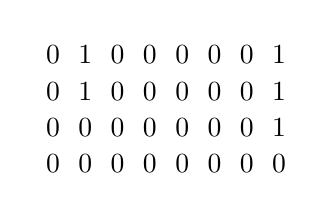
\begin{tikzpicture}
\matrix[matrix of nodes]
{
0 & 1 & 0 & 0 & 0 & 0 & 0 & 1\\
0 & 1 & 0 & 0 & 0 & 0 & 0 & 1\\
0 & 0 & 0 & 0 & 0 & 0 & 0 & 1\\
0 & 0 & 0 & 0 & 0 & 0 & 0 & 0\\
};
\end{tikzpicture}
\end{figure}
\textbf{Output}: 10
\\
\textbf{Explanation}:
\\
There are 2 contaminated regions. On the first day, add 5 walls to quarantine the viral region on the left. The board after the virus spreads is:
\begin{figure}[H]
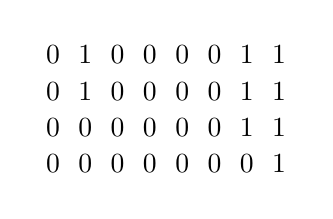
\begin{tikzpicture}
\matrix[matrix of nodes]
{
0 & 1 & 0 & 0 & 0 & 0 & 1 & 1\\
 0 & 1 & 0 & 0 & 0 & 0 & 1 & 1\\
 0 & 0 & 0 & 0 & 0 & 0 & 1 & 1\\
 0 & 0 & 0 & 0 & 0 & 0 & 0 & 1\\
};
\end{tikzpicture}
\end{figure}
On the second day, add 5 walls to quarantine the viral region on the right. The virus is fully contained.
\end{flushleft}
\paragraph{Example 2:}
\begin{flushleft}
\textbf{Input}:
\begin{figure}[H]
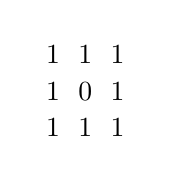
\begin{tikzpicture}
\matrix[matrix of nodes]
{
1 & 1 & 1\\
1 & 0 & 1\\
1 & 1 & 1\\
};
\end{tikzpicture}
\end{figure}
\textbf{Output}: 4
\\
\textbf{Explanation}: 
\\
Even though there is only one cell saved, there are 4 walls built.
\\
Notice that walls are only built on the shared boundary of two different cells.
\end{flushleft}
\paragraph{Example 3:}
\begin{flushleft}
\textbf{Input}:
\begin{figure}[H]
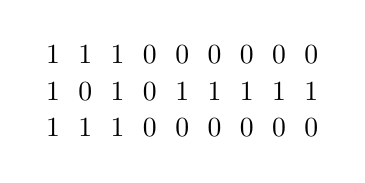
\begin{tikzpicture}
\matrix[matrix of nodes]
{
1 & 1 & 1 & 0 & 0 & 0 & 0 & 0 & 0\\
1 & 0 & 1 & 0 & 1 & 1 & 1 & 1 & 1\\
1 & 1 & 1 & 0 & 0 & 0 & 0 & 0 & 0\\
};
\end{tikzpicture}
\end{figure}
\textbf{Output}: 13
\\
\textbf{Explanation}: The region on the left only builds two new walls.
\end{flushleft}



\end{document}



